\section{Sreality.cz}
\label{analyza:sreality}
Realitní agentura Sreality.cz \cite{sreality} vytvořila webovou aplikaci, která má ulehčovat uživatelům výběr domu či bytu, ve kterém stráví následující roky svého života. Takové rozhodnutí bývá velmi náročné a proto od Sreality.cz můžeme očekávat jasné podání informací a hlavně přijatelné uživatelské prostředí. Toto očekávání je znásobené ještě tím, že uživatelé, kteří navštíví danou stránku, mohou být z~různých věkových skupin.

\subsection{Hlavní stránka}
Viz obrázek \ref{fig:sreality:homepage}.
\begin{figure}[h]
    \centering
    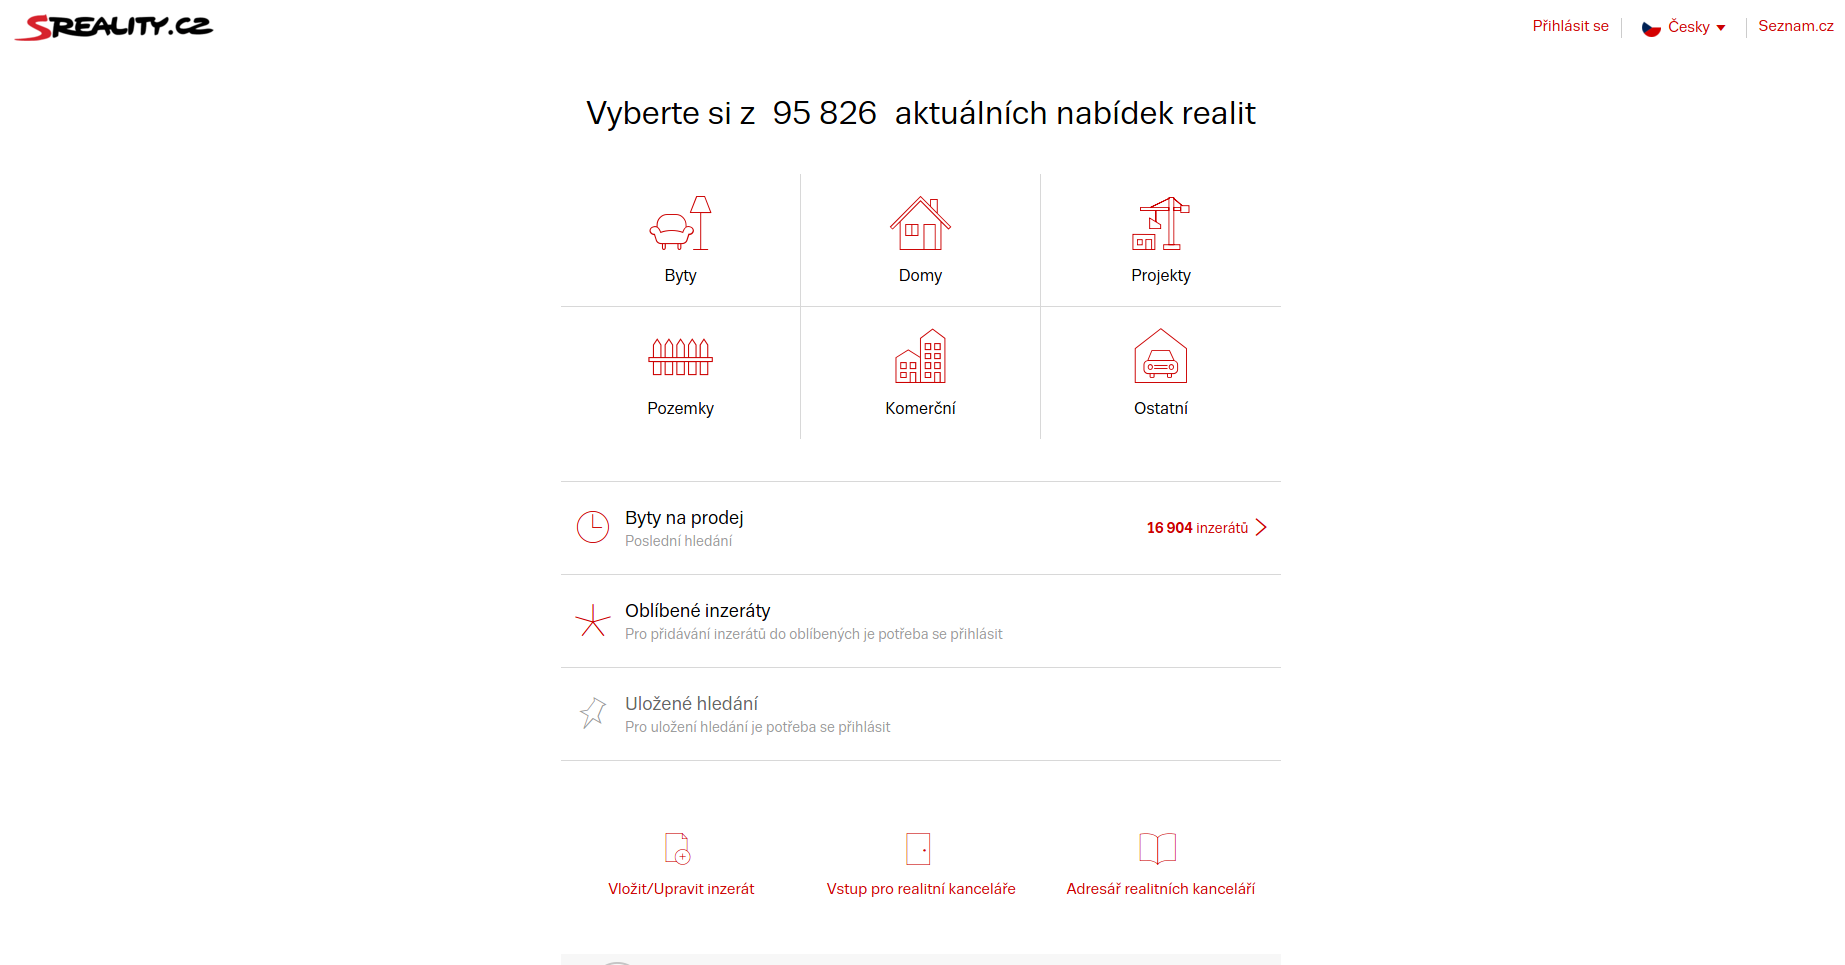
\includegraphics[width=1.0\textwidth]{media/sreality/homepage.png}
    \caption{Sreality.cz -- Hlavní stránka}
    \label{fig:sreality:homepage}
\end{figure}
\subsubsection*{Pozitiva}
\begin{itemize}
    \item[+] \textbf{Jednoduchost} -- Bílé prostředí, které obsahuje pouze černé nápisy a červené obrysové nákresy. Velmi jednoduché a přehledné řešení.
    \item[+] \textbf{Poslední a oblíbené vyhledávání} -- Speciální možnosti, které ulehčí hledání uživatelům, kteří již na dané stránce byli a pravděpodobně si již nějaké nabídky vybrali.
\end{itemize}
\subsubsection*{Negativa}
\begin{itemize}
    \item[-] \textbf{Žádná negativa na této stránce nejsou pozorována.}
\end{itemize}


%%%%%%%%%%%%%%%%%%%%%%%%%%%%%%%%%%%%%%%%%%%%%%%%%%%%%%%%%%%%%%%%%%%%%%%%%%%%%%%%%%%%%%%%%%%%%%%%%%%%%%%%%%%%%%%%%%%%%%%%

\newpage
\subsection{Vyhledávání realit}
Viz obrázky \ref{fig:sreality:detail} a \ref{fig:sreality:detail-big-map}.
\begin{figure}[h]
    \centering
    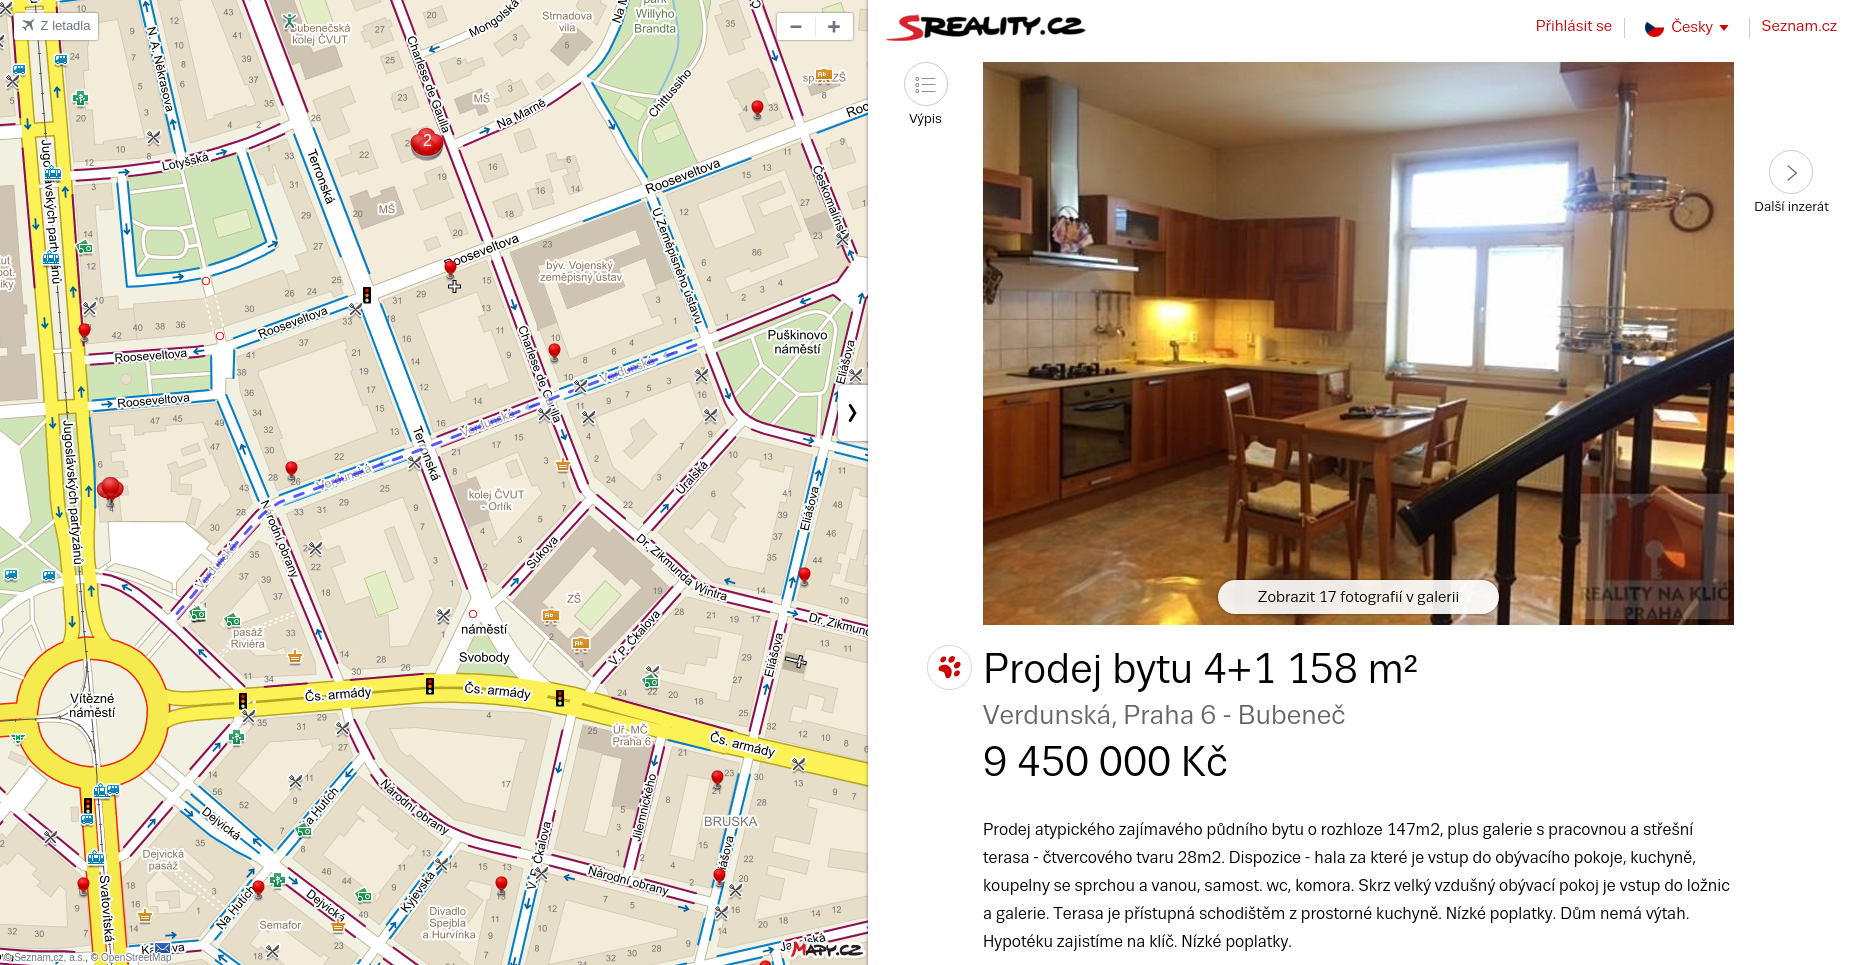
\includegraphics[width=1.0\textwidth]{media/sreality/detail.png}
    \caption{Sreality.cz -- Detail nabídky}
    \label{fig:sreality:detail}
\end{figure}
\begin{figure}[h]
    \centering
    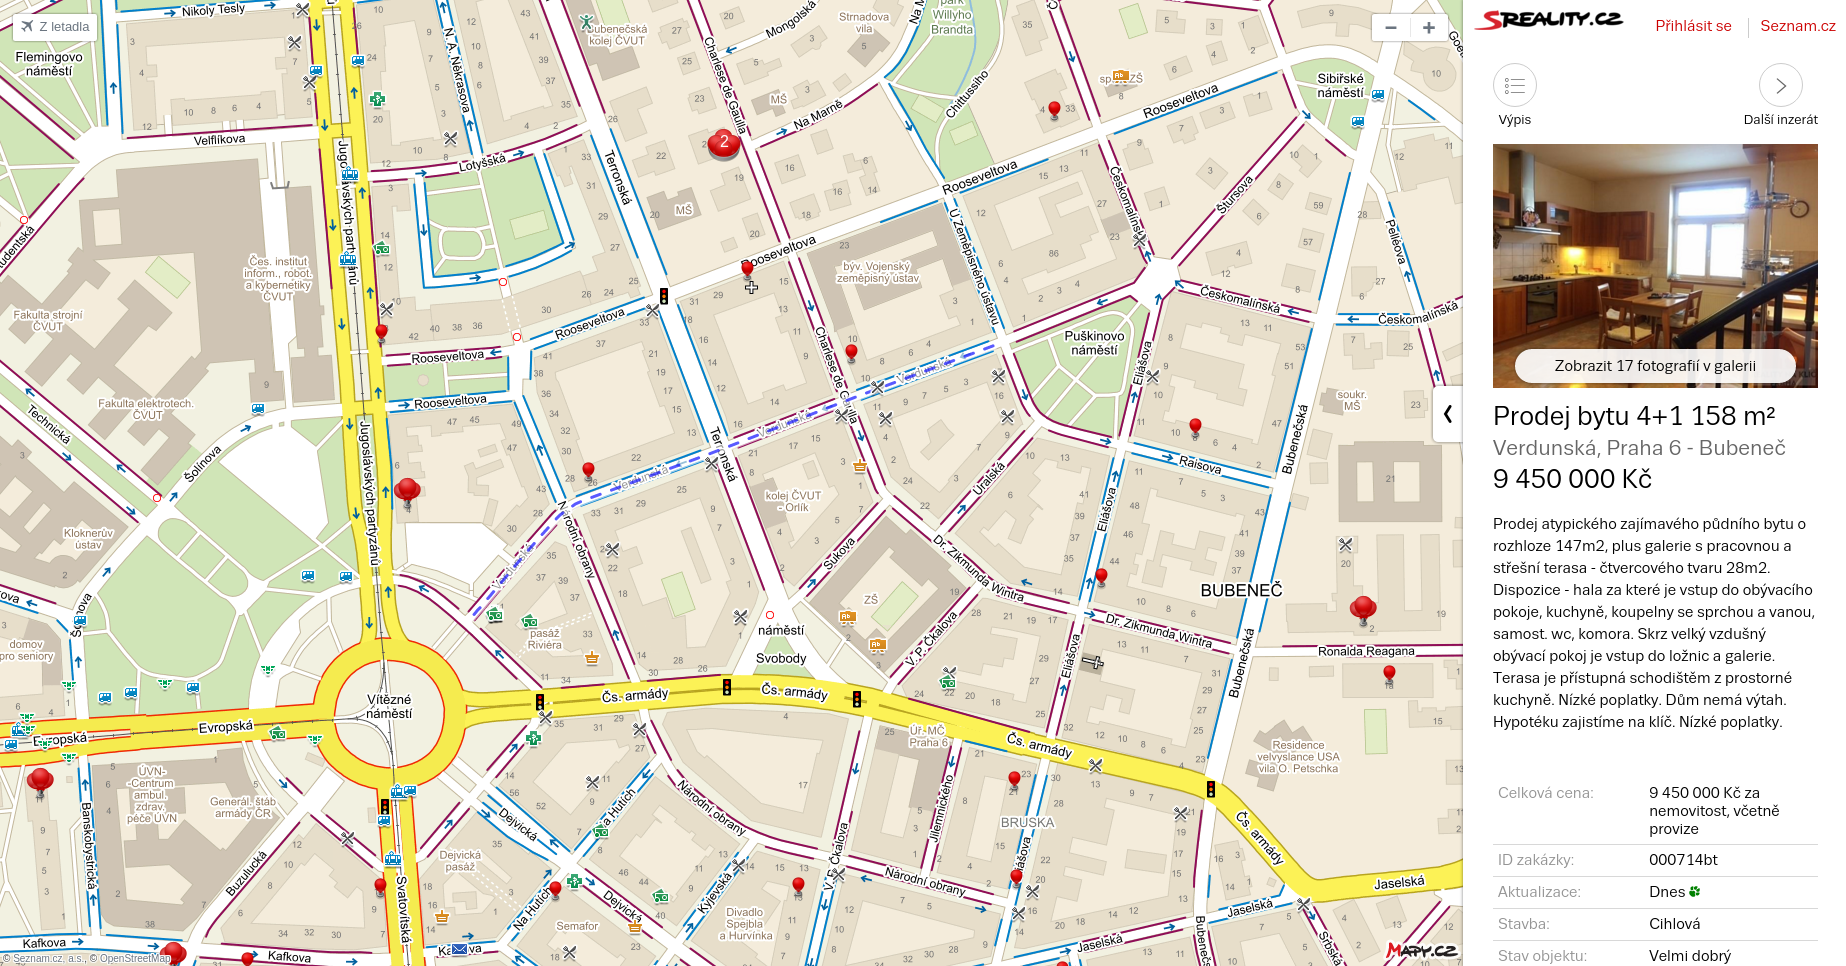
\includegraphics[width=1.0\textwidth]{media/sreality/detail-big-map.png}
    \caption{Sreality.cz -- Detail nabídky -- větší mapa}
    \label{fig:sreality:detail-big-map}
\end{figure}
\subsubsection*{Pozitiva}
\begin{itemize}
    \item[+] \textbf{Mapa} -- Krásné propojení map od společnosti Seznam.cz a vyhledávání. Navíc je hned vidět jak daleko se nachází zastávka městské hromadné dopravy nebo nejbližší supermarket a další.
    \item[+] \textbf{Lišta s~náhledem nabídky} -- Informativní popis všech vlastností dané nabídky.
    \item[+] \textbf{Zvětšení/zmenšení} -- Uživatel má možnost zvětšit, nebo zmenšit mapu a tím pádem vidět méně či naopak více z~obsahu.
\end{itemize}
\subsubsection*{Negativa}
\begin{itemize}
    \item[-] \textbf{Nemožnost čistého náhledu bez mapy} -- Při užším a delším vybírání je možné, že uživatel má lokalitu dobře zmapovanou a tím pádem nepotřebuje vidět mapu (ani v~malé formě) na levé straně obrazovky.
\end{itemize}

%%%%%%%%%%%%%%%%%%%%%%%%%%%%%%%%%%%%%%%%%%%%%%%%%%%%%%%%%%%%%%%%%%%%%%%%%%%%%%%%%%%%%%%%%%%%%%%%%%%%%%%%%%%%%%%%%%%%%%%%

\subsection{Shrnutí}
Nejzajímavějším aspektem Sreality.cz se jeví přítomnost \textbf{mapy}, která ulehčuje a urychluje výběr. Tato vlastnost bude zakomponována do webové aplikace realizované v~této práci. Forma přepínání mezi mapou a obsahem je řešená \textbf{jednoduše} a uživatelsky přijatelně.

Hodnocení uživatelů zde není nijak řešené.